\documentclass[aspectratio=169,t]{beamer}

% Some default packages
\usepackage[english]{babel}
\usepackage[utf8]{inputenc}
\usepackage[T1]{fontenc}
\usepackage{qrcode}
\usepackage{tikz}
\usetikzlibrary{shapes.geometric}
\usepackage{pgfplots}
\usepackage{pgfplotstable}

%\pgfplotsset{compat=1.9,
	%title style={color=dlrdarkblue},
	%tick label style = {color=dlrdarkblue},
	%every axis label = {color=dlrdarkblue},
	%legend style,
	%label style = {color=dlrdarkblue}
%}
%\tikzset{cross/.style={cross out, draw=black, minimum size=2*(#1-\pgflinewidth), inner sep=0pt, outer sep=0pt},
	%default radius will be 1pt. 
	%cross/.default={1pt}}

% DLR Layout
%\usetheme[beamertools={fixblocktitle=false}, professionalfonts]{dlr}
%Select Blue, Green or Yellow as color
\usetheme[helvetica,nobeamertools,nonavigation,color=Blue]{Boadilla}

% Load a color scheme for blocks
\usecolortheme{orchid}

% Titel and author
\title{Wasserstoff für Deutschland}
\subtitle{} 
\date{29.02.2024}
\author{}
\setbeamertemplate{navigation symbols}{}


% Add additional logo
%\addlogoFL{{\includegraphics[height=24pt]{UzK_black.png}}}
%\addlogoTP{{\includegraphics[height=40pt]{UzK_black.png}}}

%%%%My colors
% SFC refienemnt colors
\definecolor{blue1}{RGB}{25,45,68}
\definecolor{blue2}{RGB}{29,51,78}
\definecolor{blue3}{RGB}{32,58,87}
\definecolor{blue4}{RGB}{36,64,97}
\definecolor{blue5}{RGB}{49,79,113}
\definecolor{blue6}{RGB}{64,94,129}
\definecolor{blue7}{RGB}{81,110,144}
\definecolor{blue8}{RGB}{100,128,160}
\definecolor{blue9}{RGB}{121,146,176}
\definecolor{blue10}{RGB}{143,166,192}
\definecolor{blue11}{RGB}{168,187,208}
\definecolor{blue12}{RGB}{195,208,223}
\definecolor{blue13}{RGB}{224,231,239}


\begin{document}
	
	% Maketitle
	\maketitle
	
	
	%---------------------------------
	

	
	%---------------------------------
	\begin{frame}
		\frametitle{Grober Überblick übers Projekt}
		\vspace*{-4mm}
		\begin{minipage}{1\linewidth}
			\begin{minipage}{.5\linewidth}
				
				\vspace*{-12mm}
				
		\begin{itemize}
			\item Wollen das beschränkte Stromnetz Deutschlands modellieren
			\vspace*{2mm}
			
			\begin{itemize}
				\item [$\rightarrow$] Um Wasserstoffnetzwerk ergänzen
			\end{itemize}
		\vspace*{2mm}
		
		\item Gefälle von Nord- zu Süddeutschland bzgl. Stromproduktion und -verbrauch
		\vspace*{2mm}
		
		\begin{itemize}
			\item [$\rightarrow$] Verteilung von importiertem Strom
		\end{itemize}
				 
		\end{itemize}
	\end{minipage}
\hfill
\begin{minipage}{.5\linewidth}
\centering
\includegraphics[width=.7\linewidth]{windkraft.jpg}

\end{minipage}
\end{minipage}	
		
			
		
	\end{frame}


		%---------------------------------
	\begin{frame}
		\frametitle{Grober Überblick übers Projekt}
		\vspace*{-4mm}
		\begin{minipage}{1\linewidth}
			\begin{minipage}{.5\linewidth}
				\vspace*{-12mm}
				
				\begin{itemize}
					
					\item Für welche Gegebenheiten lohnt sich dieses Wasserstoffnetz?
						\vspace*{2mm}
					
					\item Aktuell: Stromtrassen als Lösung
						\vspace*{2mm}
					
					\item Problem: ungenutzter Strom 
						\vspace*{2mm}
					
					\item Lösung: Strom in Form von Wasserstoff speichern und transportieren 
					
					
				\end{itemize}
			\end{minipage}
			\hfill
			\begin{minipage}{.5\linewidth}
				\centering
				\includegraphics[width=.7\linewidth]{windkraft.jpg}
				
			\end{minipage}
		\end{minipage}	
		
		
		
	\end{frame}
	
	%---------------------------------
	
	\begin{frame}
		\frametitle{Erste Schritte}
		\vspace*{0mm}
		\begin{minipage}{1\linewidth}
			\begin{minipage}{.5\linewidth}
				\begin{itemize}
					\item Modellierung des Stromnetzes in Deutschland
					\item Bundesländer als Knoten eines gerichteten Graphens in Python
					\item einfaches Beispiel mit vereinfachten Annahmen
					\item ausschließlich Sonnen- und Windenergie
				\end{itemize}
			\end{minipage}
			\hfill
			\begin{minipage}{.5\linewidth}
				\centering
				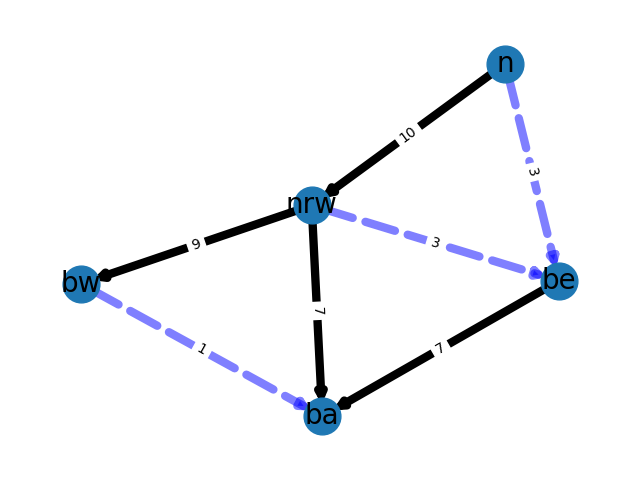
\includegraphics[width=.7\linewidth]{Example_graph.png}
				
			\end{minipage}
		\end{minipage}	
		
	\end{frame}

	%---------------------------------
% \begin{frame}
% 	\frametitle{Annahmen}
% 	\vspace*{0mm}
% 	\begin{minipage}{1\linewidth}
% 		\begin{minipage}{.3\linewidth}
% 			\begin{itemize}
% 				\item Verbrauch
% 				\item 1 toe = 11.63 megawatt-hours (MWh)
% 			\end{itemize}
% 		\end{minipage}
% 		\hfill
% 		\begin{minipage}{.7\linewidth}
% 			\centering
% 			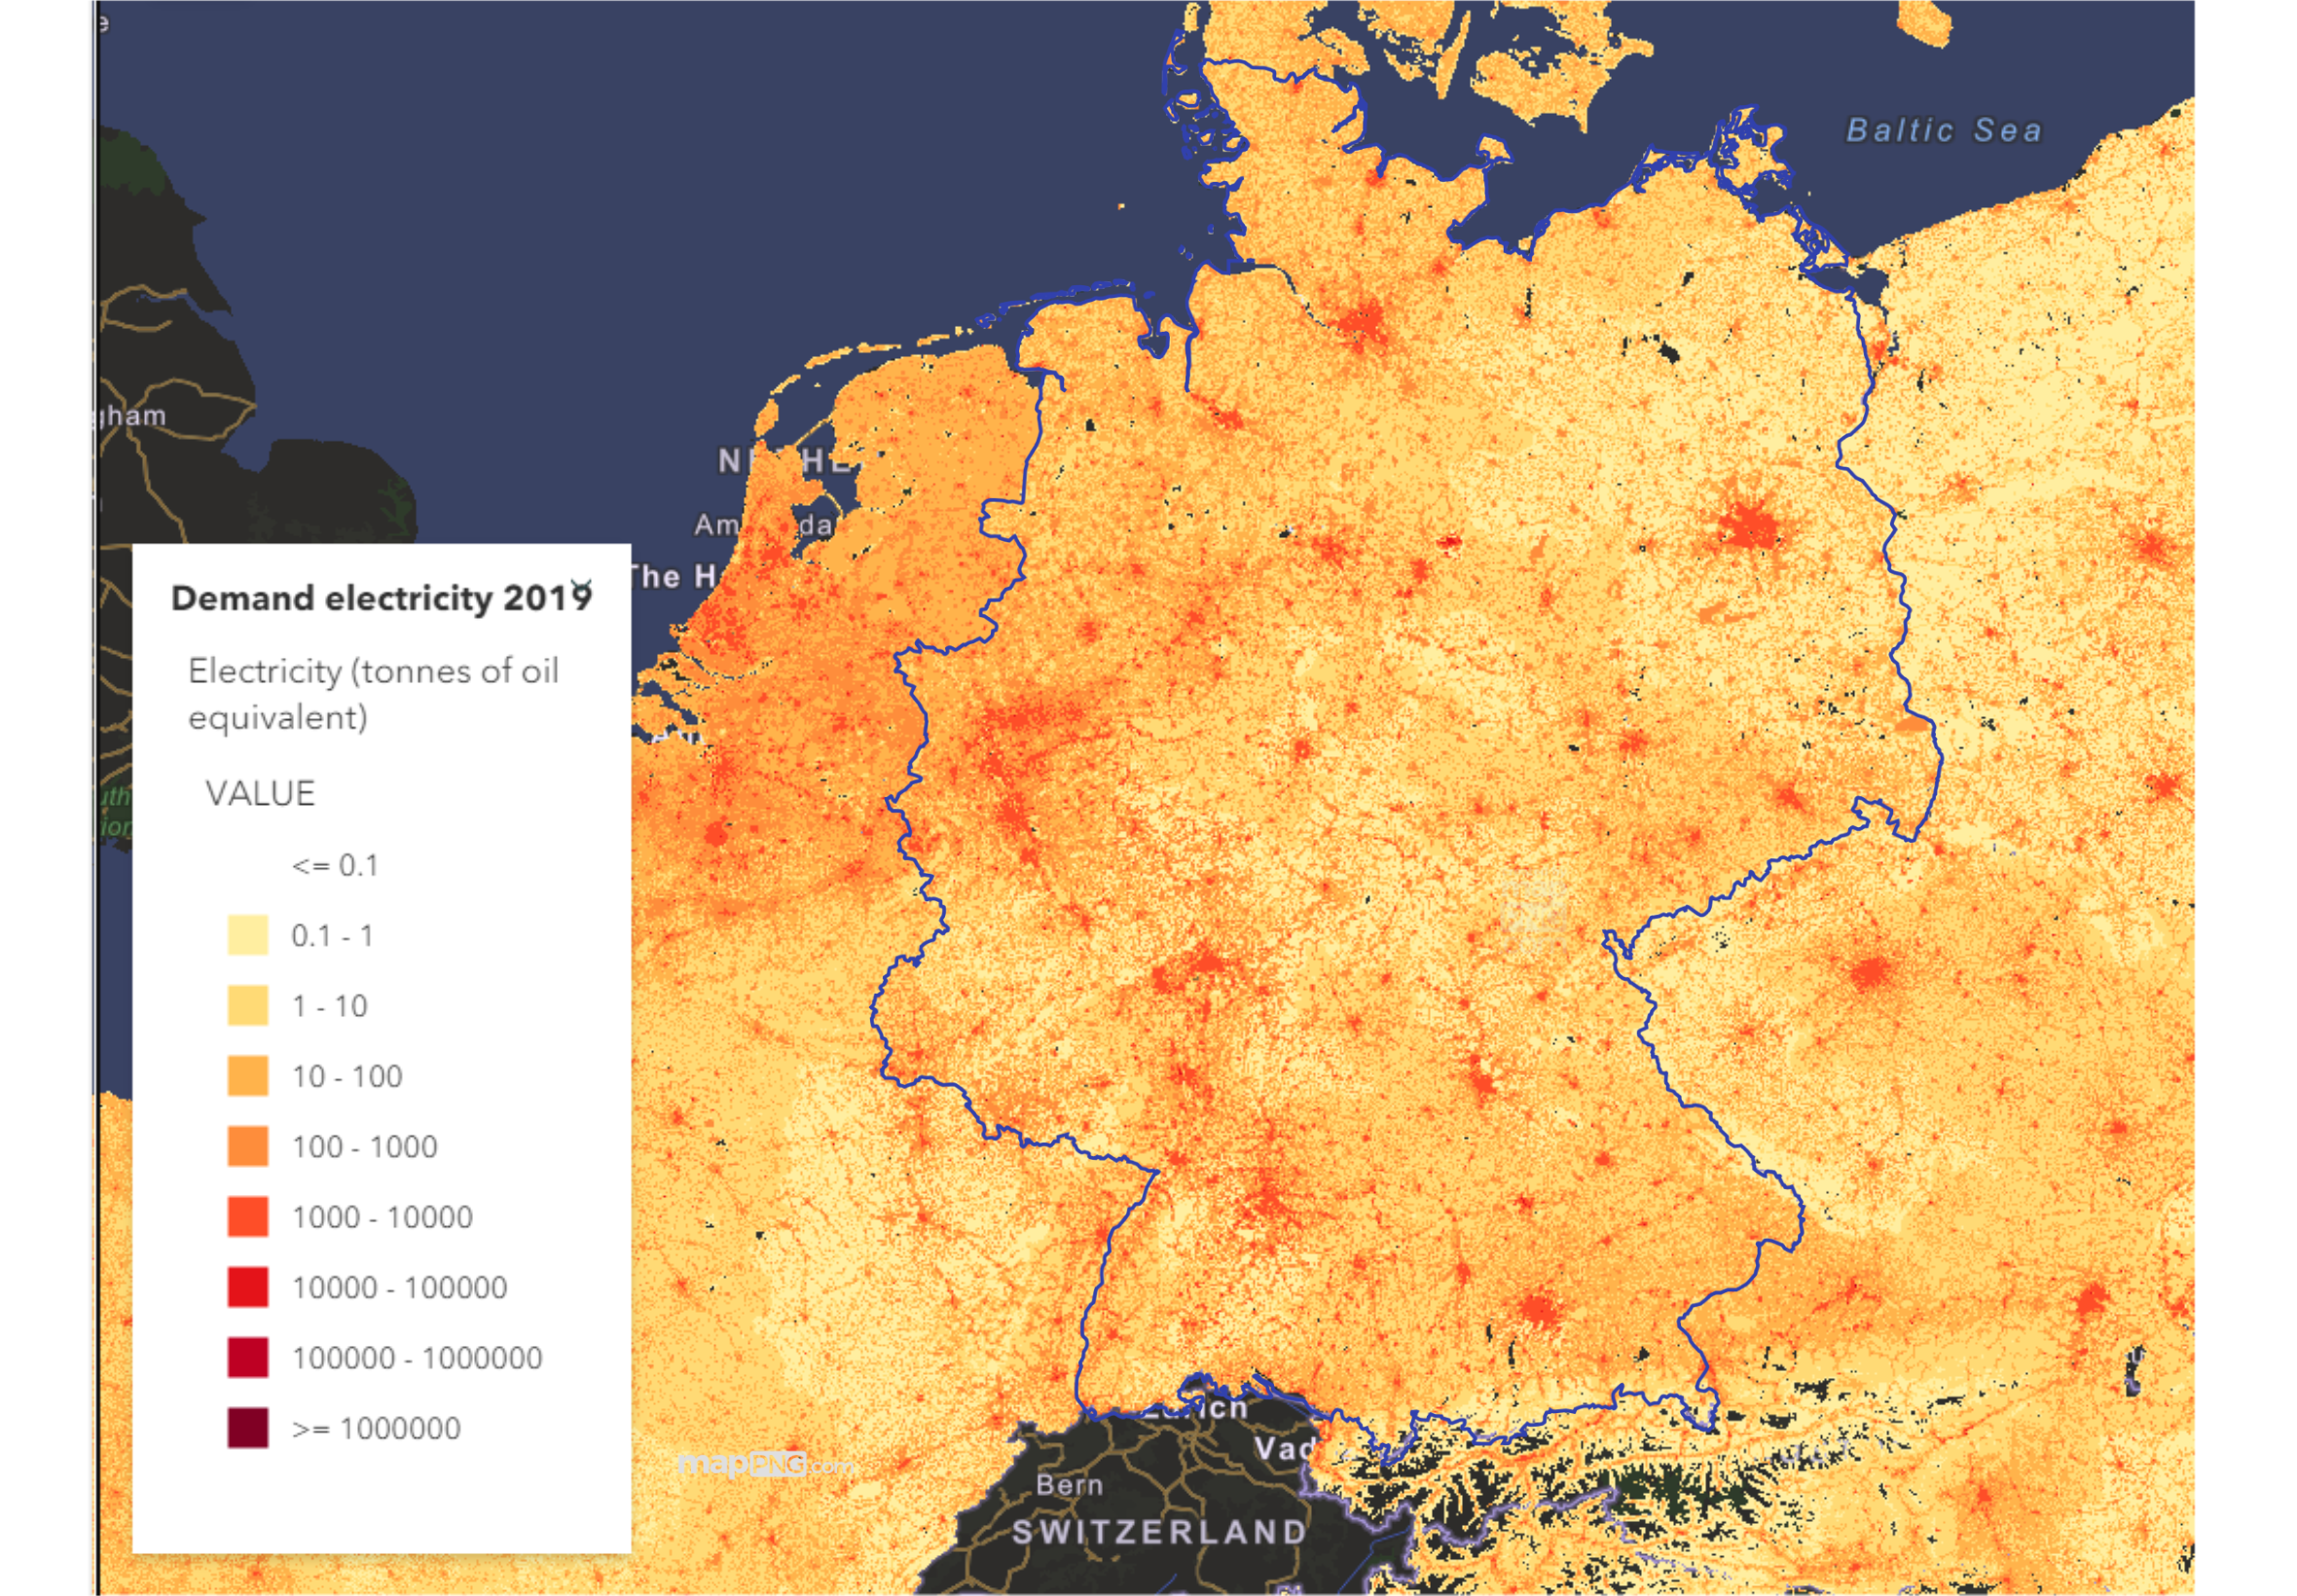
\includegraphics[width=.9\linewidth]{Deutschland_Bedarf.png}
			
% 		\end{minipage}
% 	\end{minipage}	

% \vspace*{4mm}
% 	Quelle: https://energy-industry-geolab.jrc.ec.europa.eu/energy-atlas/
	
% \end{frame}

	%---------------------------------


% \begin{frame}
% 	\frametitle{}
	
% 	\vspace*{-2mm}
% 	%Verbrauch: https://www.statistikportal.de/de/ugrdl/ergebnisse/energie/pev#5238
% 	%Erzeugung: https://www.statistikportal.de/de/ugrdl/ergebnisse/energie/swe#5897
% 	\vspace*{0mm}
% \end{frame}
%---------------------------------
	

	%---------------------------------
	\begin{frame}
		\frametitle{Weitere Vorgehensweise}
		\vspace*{0mm}
			\begin{minipage}{1\linewidth}
			\begin{minipage}{.5\linewidth}
				\begin{itemize}
					\item ursprüngliche Idee: Deutschland aufgeteilt in 16 Bundesländer
					\item kleines Problem: Zeitreihendaten nicht ohne Weiteres verfügbar
					\item großes Problem: Keine gute Datensätze für Trassen zwischen Bundesländern
					\item Idee: Kleinskaliger mit SMARD-Daten für die vier Regelzonen arbeiten
					\item auch nicht wirklich gut: Zu Verbrauch/Produktion gibt es gute Daten, aber die Übertragung zwischen Netzen wird nicht abgebildet
					\item Datenportal zur aktuellen FfE-Studie nicht verfügbar
				\end{itemize}
			\end{minipage}
			\hfill
			\begin{minipage}{.5\linewidth}
				\centering
				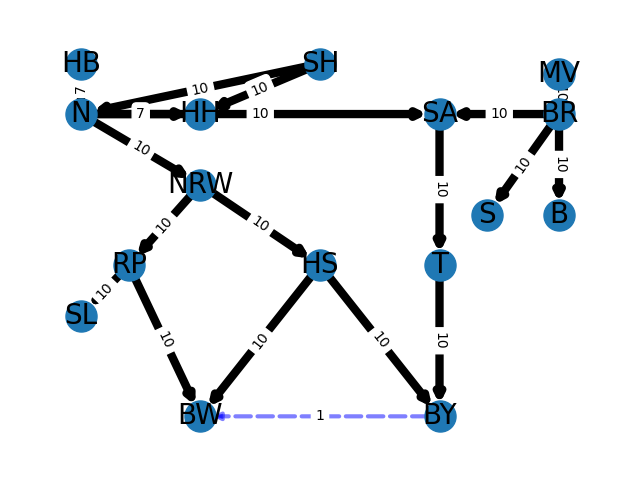
\includegraphics[width=.8\linewidth]{Example_graph_2.png}
				
			\end{minipage}
		\end{minipage}	
	
			
	\end{frame}
	%---------------------------------
	
	\begin{frame}
		\frametitle{Daten: Open­Energy­Platform}
		\begin{itemize}
			\item große, offene Datenbank mit REST API
			\item wir nutzen Daten, die auch für eTraGo-Paket (Transmission grid optimization) genutzt werden
			\item ausreichend, um Hochspannungsnetz über ein Jahr zu modellieren
			\item grid-Daten (ergo Standort/Geometrie) zu
			\begin{itemize}
				\item bus (Sammelschiene)
				\item generator (Kraftwerke)
				\item load (Verbrauch/Nachfrage)
				\item storage (Speicher)
				\item transformer (Wandler)
				\item line (Stromtrasse)
			\end{itemize}
			\item Zeitreihendaten (ein Jahr viertelstündlich?) für
			\begin{itemize}
				\item load 
				\item generator (sehr groß; gefiltertes JSON ca. $3{,}7$ GB)
			\end{itemize}
			\item eTraGo verwendet PyPSA (Python-Paket), werden wir voraussichtlich auch benutzen
		\end{itemize}
	\end{frame}
	
	\begin{frame}
		\frametitle{Daten: Generierung}
		\begin{itemize}
			\item OpenStreetMap wird häufig für Erstellung von Stromnetzdaten genutzt
			\item Nachfragezeitreihe mittels Standardlastprofil erstellt
			\item Zeitbezug für Version nicht ganz klar, aber wohl aktuell
			\item man kann wohl komplette Datenbank über GitHub nachbauen, aber sehr aufwändig
			\item genutzt wird in der Datenbank PostgreSQL, wir werden wahrscheinlich ein Format wie HDF5 nutzen, falls Zeitreihen angewendet werden
		\end{itemize}
	\end{frame}

	\begin{frame}
		\frametitle{Beispielplot: Stromtrassen}
		\vspace*{-1.3cm}
		\hspace*{6cm}
		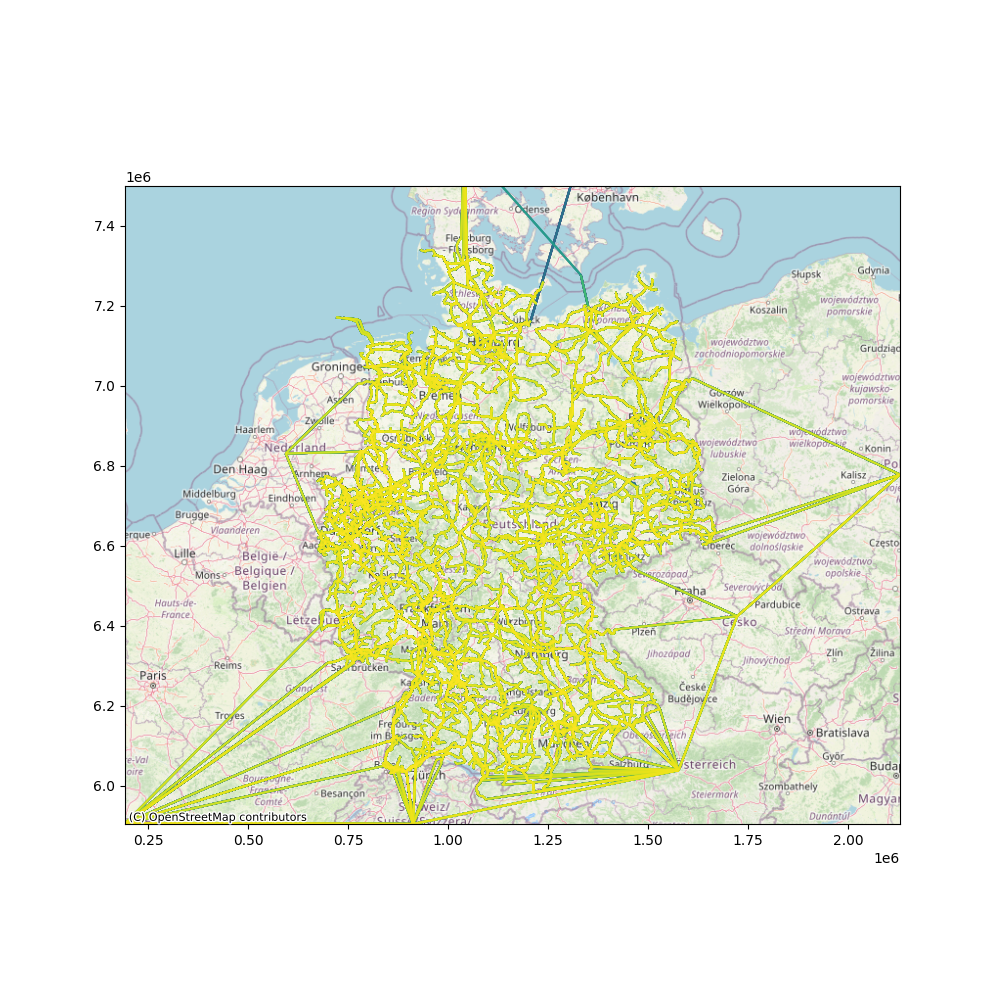
\includegraphics[height=10cm]{./line.png}
	\end{frame}

	\begin{frame}
		\frametitle{Herleitung der Powerflow Equations}
		
	\end{frame}
	%---------------------------------
	
	

	
	
	\begin{frame}
		\frametitle{Ausblick}
		
		\vspace*{6mm}
		\begin{itemize}
			\item erste praktische Versuche mit PyPSA bzw. Lastflussberechnungen
			\item weitere Daten suchen:
			\begin{itemize}
				\item Gasnetz (eventuell über entsog transparency platform),
				\item Bauvorhaben Wasserstoff
			\end{itemize}
			\item Kostenmodell aufstellen
			\item Unsere Stromdaten liefern verschiedene Szenarien zur Energiewende:
			
			Vielleicht reicht das für Erzeugung schon aus? 
			\item Wie genau funktioniert Import/Export?
			% \item Stahlindustrie betrachten
		\end{itemize}
			
		
	\end{frame}
	
	
	
	%---------------------------------
	
	
	
	
\end{document}
% eof
